\documentclass[spanish,a4paper,11pt,twoside]{report}

%%%%%%%%%%%%%%%%%%%%%%%%%%%%%%%%%%%%%%%%%%%%%%%%%%%%%%%%%%%%%%%%%%%%%%%%%%%%%%%
\usepackage[dvips]{graphicx}
\usepackage[dvips]{epsfig}
\usepackage[utf8]{inputenc}
\usepackage[spanish]{babel}
\usepackage{alltt}
\usepackage{templates/algorithm}
\usepackage{templates/algorithmic}
\usepackage{templates/multirow}

%%%%%%%%%%%%%%%%%%%%%%%%%%%%%%%%%%%%%%%%%%%%%%%%%%%%%%%%%%%%%%%%%%%%%%%%%%%%%%%

\newcommand{\SONY}{{\sc Sony}}
\newcommand{\MICROSOFT}{{\sc Microsoft}}
\newcommand{\GCC}{\textsf{\textsc{G}CC}}
\newcommand{\INTEL}{\textsf{\textsc{I}ntel}}

%%% Traducimos el pseudocodigo
\renewcommand{\algorithmicwhile}{\textbf{mientras}}
\renewcommand{\algorithmicend}{\textbf{fin}}
\renewcommand{\algorithmicdo}{\textbf{hacer}}
\renewcommand{\algorithmicif}{\textbf{si}}
\renewcommand{\algorithmicthen}{\textbf{entonces}}
\renewcommand{\algorithmicrepeat}{\textbf{repetir}}
\renewcommand{\algorithmicuntil}{\textbf{hasta que}}
\renewcommand{\algorithmicelse}{\textbf{en otro caso}}
\renewcommand{\algorithmicfor}{\textbf{para}}

%\newcommand{\RETURN}{\textbf{retornar} }
\newcommand{\RET}{\STATE \textbf{retornar} }
\newcommand{\TO}{\textbf{hasta} }
\newcommand{\AND}{\textbf{y} }
\newcommand{\OR}{\textbf{o} }

%%%%%%%%%%%%%%%%% Creamos un entorno para listar código fuente %%%%%%%%%%%%%%%
\newenvironment{sourcecode}
{\begin{list}{}{\setlength{\leftmargin}{1em}}\item\scriptsize\bfseries}
{\end{list}}

\newenvironment{littlesourcecode}
{\begin{list}{}{\setlength{\leftmargin}{1em}}\item\tiny\bfseries}
{\end{list}}

\newenvironment{summary}
{\par\noindent\begin{center}\textbf{Abstract}\end{center}\begin{itshape}\par\noindent}
{\end{itshape}}

\newenvironment{keywords}
{\begin{list}{}{\setlength{\leftmargin}{1em}}\item[\hskip\labelsep \bfseries Keywords:]}
{\end{list}}

\newenvironment{palabrasClave}
{\begin{list}{}{\setlength{\leftmargin}{1em}}\item[\hskip\labelsep \bfseries Palabras clave:]}
{\end{list}}


%%%%%%%%%%%%%%%%%%%%%%%%%%%%%%%%%%%%%%%%%%%%%%%%%%%%%%%%%%%%%%%%%%%%%%%%%%%%%%%
% Format
%%%%%%%%%%%%%%%%%%%%%%%%%%%%%%%%%%%%%%%%%%%%%%%%%%%%%%%%%%%%%%%%%%%%%%%%%%%%%%%

%%\topmargin -4 mm
%\topmargin -21 mm
%\headheight 10 mm
%\headsep 10 mm

%\textheight 229 mm
%\textheight 246 mm

%\oddsidemargin -5.4 mm
%\evensidemargin -5.4 mm
\oddsidemargin 5 mm
\evensidemargin 5 mm

%\oddsidemargin -3 mm
%\evensidemargin -3 mm

%\textwidth 17 cm
\textwidth 15 cm
%\columnsep 10 mm

\input{amssym.def}

%%%%%%%%%%%%%%%%%%%%%%%%%%%%%%%%%%%%%%%%%%%%%%%%%%%%%%%%%%%%%%%%%%%%%%%%%%%%%%%

\begin{document}

%%%%%%%%%%%%%%%%%%%%%%%%%%%%%%%%%%%%%%%%%%%%%%%%%%%%%%%%%%%%%%%%%%%%%%%%%%%%%%%
% First Page 
%%%%%%%%%%%%%%%%%%%%%%%%%%%%%%%%%%%%%%%%%%%%%%%%%%%%%%%%%%%%%%%%%%%%%%%%%%%%%%%

\pagestyle{empty}
\thispagestyle{empty}


\newcommand{\HRule}{\rule{\linewidth}{1mm}}
\setlength{\parindent}{0mm}
\setlength{\parskip}{0mm}
\vspace*{\stretch{1}}

\begin{center}

\includegraphics[width=0.2\textwidth]{images/logotipo-secundario-ULL}\\[0.25cm]
\end{center}

\HRule
\begin{center}
        {\Huge Series de potencias: Newton} \\[2.5mm] 
        {\Huge f(x)= sin(x)} \\[2.5mm]
        {\Large Zoilo González Garcia} \\[5mm]
        {\Large  Francisco Javier Reyes Sánchez} \\[5mm]
        {\Large \textit{Grupo ($2ºE$) }} \\[5mm]


        {\em Técnicas Experimentales. $1^{er}$ curso. $2^{do}$ cuatrimestre} \\[5mm]
        Lenguajes y Sistemas Informáticos \\[5mm]
        Facultad de Matemáticas \\[5mm]
        
        Universidad de La Laguna \\
\end{center}
\HRule
\vspace*{\stretch{2}}
\begin{center}
  La Laguna, \today 
\end{center}

%%%%%%%%%%%%%%%%%%%%%%%%%%%%%%%%%%%%%%%%%%%%%%%%%%%%%%%%%%%%%%%%%%%%%%%%%%%%%%%

%%%%%%%%%%%%%%%%%%%%%%%%%%%%%%%%%%%%%%%%%%%%%%%%%%%%%%%%%%%%%%%%%%%%%%%%%%%%%%%
\newpage{\pagestyle{empty}\cleardoublepage}

\pagestyle{myheadings} %my head defined by markboth or markright
% No funciona bien \markboth sin "twoside" en \documentclass, pero al
% ponerlo se dan un montón de errores de underfull \vbox, con lo que no se
% ha puesto.
\markboth{Francisco Reyes y Zoilo González}{Series de potencias: Newton}

%%%%%%%%%%%%%%%%%%%%%%%%%%%%%%%%%%%%%%%%%%%%%%%%%%%%%%%%%%%%%%%%%%%%%%%%%%%%%%%
%Numeracion en romanos
\renewcommand{\thepage}{\roman{page}}
\setcounter{page}{1}

%%%%%%%%%%%%%%%%%%%%%%%%%%%%%%%%%%%%%%%%%%%%%%%%%%%%%%%%%%%%%%%%%%%%%%%%%%%%%%%

\tableofcontents

%%%%%%%%%%%%%%%%%%%%%%%%%%%%%%%%%%%%%%%%%%%%%%%%%%%%%%%%%%%%%%%%%%%%%%%%%%%%%%%
\newpage{\pagestyle{empty}\cleardoublepage}

\listoffigures

%%%%%%%%%%%%%%%%%%%%%%%%%%%%%%%%%%%%%%%%%%%%%%%%%%%%%%%%%%%%%%%%%%%%%%%%%%%%%%%
\newpage{\pagestyle{empty}\cleardoublepage}

\listoftables

%%%%%%%%%%%%%%%%%%%%%%%%%%%%%%%%%%%%%%%%%%%%%%%%%%%%%%%%%%%%%%%%%%%%%%%%%%%%%%%
\newpage{\pagestyle{empty}\cleardoublepage}

%%%%%%%%%%%%%%%%%%%%%%%%%%%%%%%%%%%%%%%%%%%%%%%%%%%%%%%%%%%%%%%%%%%%%%%%%%%%%%%
%Numeracion a partir del capitulo I
\renewcommand{\thepage}{\arabic{page}}
\setcounter{page}{1}

\setlength{\parindent}{5mm}

%%%%%%%%%%%%%%%%%%%%%%%%%%%%%%%%%%%%%%%%%%%%%%%%%%%%%%%%%%%%%%%%%%%%%%%%%%%%%%%
\chapter{Motivación y objetivos}
\label{chapter:obj}

 %%%%%%%%%%%%%%%%%%%%%%%%%%%%%%%%%%%%%%%%%%%%%%%%%%%%%%%%%%%%%%%%%%%%%%%%%%%%%
% Chapter 1: Motivación y Objetivos
%%%%%%%%%%%%%%%%%%%%%%%%%%%%%%%%%%%%%%%%%%%%%%%%%%%%%%%%%%%%%%%%%%%%%%%%%%%%%%%

Los objetivos para los que se plantea este trabajo, son el adquirir conocimientos y mejorar nuestras habilidades en el uso del lenguaje de programanción PYTHON, procesador de texto \LaTeX{} y una clase de \LaTeX{} que nos permite diseñar presentaciones, BEAMER. Además, desde un punto de vista matemático, aprenderemos el método de Interpolación Polinómica de Newton para la aproximación de una función en un intervalo determinado, haciendo uso de las diferencias divididas de Newton.
%---------------------------------------------------------------------------------
\section{Sección Uno: \LaTeX}
\label{1:sec:1}
 Es un sistema de composición muy adecuado para realizar documentos científicos y matemáticos de alta calidad tipográfica. Es también adecuado para producir documentos de cualquier otro tipo, desde simples cartas a libros enteros.\par\LaTeX{} está formado mayoritariamente por órdenes construidas a partir de comandos de \TeX{} (lenguaje de nivel bajo), en el sentido de que sus acciones son muy elementales, pero con la ventaja añadida de poder aumentar las capacidades de \LaTeX{} utilizando comandos propios del \TeX{} descritos en The TeXbook.3 4. Esto es lo que convierte a \LaTeX{} en una herramienta práctica y útil pues, a su facilidad de uso, se une toda la potencia de \TeX{}. Estas características hicieron que \LaTeX{} se extendiese rápidamente entre un amplio sector científico y técnico, hasta el punto de convertirse en uso obligado en comunicaciones y congresos, y requerido por determinadas revistas a la hora de entregar artículos académicos.
%---------------------------------------------------------------------------------
\section{Sección Dos: BEAMER}
\label{1:sec:2}
El nombre viene del vocablo alemán "beamer", un pseudo-anglicismo que significa videoproyector. BEAMER es una clase de \LaTeX{} para la creación de presentaciones. Funciona con pdflatex, dvips y LyX.\par Al estar basado en LaTeX, Beamer es especialmente útil para preparar presentaciones en las que es necesario mostrar gran cantidad de expresiones matemáticas, el fuerte de dicho sistema de maquetación.


%%%%%%%%%%%%%%%%%%%%%%%%%%%%%%%%%%%%%%%%%%%%%%%%%%%%%%%%%%%%%%%%%%%%%%%%%%%%%%%
\chapter{Fundamentos teóricos}
\label{chapter:teo}

%%%%%%%%%%%%%%%%%%%%%%%%%%%%%%%%%%%%%%%%%%%%%%%%%%%%%%%%%%%%%%%%%%%%%%%%%%%%%%%
% Chapter 2: Fundamentos Teóricos 
%%%%%%%%%%%%%%%%%%%%%%%%%%%%%%%%%%%%%%%%%%%%%%%%%%%%%%%%%%%%%%%%%%%%%%%%%%%%%%%

%++++++++++++++++++++++++++++++++++++++++++++++++++++++++++++++++++++++++++++++


%++++++++++++++++++++++++++++++++++++++++++++++++++++++++++++++++++++++++++++++

\section{Interpolación Polinómica}
\label{2:sec:1}
En análisis numérico, la interpolación polinomial es una técnica de interpolación de un conjunto de datos o de una función por un polinomio. Es decir, asumimos que sólo se conoce la imagen de una función en un número finito de abscisas. En muchos de los casos, ni siquiera se conocerá la expresión de la función.\par El objetivo de esta técnica es el de hallar un polinomio que tome los valores antes mencionados y que permita hallar aproximaciones de valores desconocidos para la función. Para segurar la precisión del polinomio se dispondrá de una fórmula del error de interpolación que permitirá ajustarlo.

\section{Cálculo del polinomio interpolador de Newton}
\label{2:sec:2}
  Existen varios métodos generales de interpolación polinómica \cite{url:interpolacion} que permiten aproximar una función por medio de un polinomio de grado m. En este informe, se recogerá exclusivamente el método de las diferencias divididas de Newton.\par Definición: Sea $f_{n}$  una variable discreta de n  elementos y sea $x_{n}$ otra variable discreta de n elementos los cuales corresponden a la imagen y la abcisa de los datos que se quieran interpolar:
  \[f(x_{k})=f_{k}, \hspace{0.5 cm} k=1,...,n\]\par
  Una gran ventaja sobre la forma clásica de Lagrange es que podemos agregar un mayor número de nodos a la tabla de datos, lo que nos facilitará en gran medida el cálculo del polinomio, sobretodo, en aquellos casos en los que el grado del polinomio que se quiere calcular es bastante elevado.\par Pongamos un ejemplo: el polinomio de grado n-1  resultante de aplicar este método, tendrá la forma:
  \[\sum_{i=0}^{n-1} {a_j}{g_j}(x)\]\par Donde:\par \[ g_{j}=\prod_{j=1}^{j-1}{(x-x_{i})}\]\par
  \[ a_{j}=f[x_{0},x_{1},...,x_{j-1},x_{j},]\]\par Los coeficientes $a_{j}$ son las llamadas diferencias divididas. El cálculo de estas diferencias es el paso que caracteriza este método. Tenemos que las diferencias divididas serían de la forma siguiente:
  
  \vspace{1.5 true cm}
  %--------------------------------------------------------------------------
\begin{table}[!ht]
\begin{center}
\begin{tabular}{|c|c|} \hline 
\textbf{Tiempo  } & \textbf{Velocidad} \\ 
\textbf{($\pm$ 0.001 s)} & \textbf{($\pm$ 0.1 m/s)} \\ \hline \hline
1.234 &
67.8
\\
\hline

2.345 &
78.9
\\
\hline

3.456 &
89.1
\\
\hline

4.567 &
91.2
\\
\hline

\end{tabular}
\end{center}
\caption{Resultados experimentales de tiempo (s) y velocidad (m/s)}
\label{tab:1}
\end{table}




%%%%%%%%%%%%%%%%%%%%%%%%%%%%%%%%%%%%%%%%%%%%%%%%%%%%%%%%%%%%%%%%%%%%%%%%%%%%%%%
\chapter{Procedimiento experimental}
\label{chapter:exp}

%%%%%%%%%%%%%%%%%%%%%%%%%%%%%%%%%%%%%%%%%%%%%%%%%%%%%%%%%%%%%%%%%%%%%%%%%%%%%%%
% Chapter 3: Procedimiento experimental 
%%%%%%%%%%%%%%%%%%%%%%%%%%%%%%%%%%%%%%%%%%%%%%%%%%%%%%%%%%%%%%%%%%%%%%%%%%%%%%%
%++++++++++++++++++++++++++++++++++++++++++++++++++++++++++++++++++++++++++++++
\section{Descripción de los experimentos}
\label{3:sec:1}
El experimento ha consistido en la implemenación en Python de algoritmos capaces de resolver el problema en cuestión. Para ello se ha creado una función cuya labor es calcular el seno dada cualquier x, otra que calcula las diferencias divididas a partir de una serie de nodos, una tercera que nos calcula el polinomio resultante que aproxima la función y por último una funcción de prueba donde se dan unos valores comprendidos en el intervalo de aproximacíon y compara su seno con el valor propuesto por nuestro polinomio.

%++++++++++++++++++++++++++++++++++++++++++++++++++++++++++++++++++++++++++++++
\section{Descripción del material}
\label{3:sec:2}
    Para la realización de este experimento el material necesario ha sido el siguiente:
 \begin{itemize}
  \item El ordenador usado en la realizacción de dicho experimento ha sido un portátil de la marca hp con un procesador Intel Atom{\tiny inside}. Este consta de 231,9 Gb de disco duro y 2 Gb de memoria RAM.
  \item El sistema operativo con el que hemos trabajado es una adaptación de la distribución de Linux \textit{kubuntu} a las necesidades en cuanto a Software de los miembros de la comunidad universitaria ULL: Bardinux \cite{url:bardinux}. 
 
  \begin{figure}
  \begin{center}
  
\includegraphics[scale=0.15]{images/bardinux.eps}
  \end{center}
  \caption{Logo Bardinux}
  \label{graph:1}
  \end{figure}
  \item También hemos hecho uso de materiales tales como calculadora, folio y lápiz, pues han habido cuestiones que han sido necesarias resolver a mano para la posterior implementación del código.
 \end{itemize}
 
%++++++++++++++++++++++++++++++++++++++++++++++++++++++++++++++++++++++++++++++
\section{Resultados obtenidos}
\label{3:sec:3}
Tras la implementación del código y la obtención del polinomio de aproximación hemos comprobado su precisión dando valores a las x y estos han sido resultados de algunos ejemplos:
\vspace{1.5 true cm}


\begin{figure}
\includegraphics[scale=0.38]{images/comprobacion.eps}
\caption{Consola}
\label{graph:2}
\end{figure}
%++++++++++++++++++++++++++++++++++++++++++++++++++++++++++++++++++++++++++++++
\section{Análisis de los resultados}
\label{3:sec:4}
A la hora de analizar la calidad de las aproximaciones dadas, se puede observar que, aunque buenas, estas no son del todo exactas. Desde un punto de vista teórico, si quisieramos unos mejores resultados en las aproximaciones, una solución efectiva sería seleccionar un mayor número de nodos. En nuestro caso el número de nodos en los que hemos dividido el intervalo $(0, \pi/2)$ es de 4: $(0, \pi/6, \pi/3, \pi/2)$; dejando entre cada uno de ellos un espacio equidistante.
Otro punto de vista a la hora de analizar los datos que hay que tener en cuenta es la calidad del material utilizado, en nuestro caso, las diferentes características de la máquina de cómputo mencionadas anteriormente.


%%%%%%%%%%%%%%%%%%%%%%%%%%%%%%%%%%%%%%%%%%%%%%%%%%%%%%%%%%%%%%%%%%%%%%%%%%%%%%%
\chapter{Conclusiones}
\label{chapter:conclusiones}

%%%%%%%%%%%%%%%%%%%%%%%%%%%%%%%%%%%%%%%%%%%%%%%%%%%%%%%%%%%%%%%%%%%%%%%%%%%%%
% Chapter 4: Conclusiones y Trabajos Futuros 
%%%%%%%%%%%%%%%%%%%%%%%%%%%%%%%%%%%%%%%%%%%%%%%%%%%%%%%%%%%%%%%%%%%%%%%%%%%%%%%

bla, bla, bla, etc.


%%%%%%%%%%%%%%%%%%%%%%%%%%%%%%%%%%%%%%%%%%%%%%%%%%%%%%%%%%%%%%%%%%%%%%%%%%%%%%%

%%%%%%%%%%%%%%%%%%%%%%%%%%%%%%%%%%%%%%%%%%%%%%%%%%%%%%%%%%%%%%%%%%%%%%%%%%%%%%%
\newpage{\pagestyle{empty}\cleardoublepage}
\thispagestyle{empty}
\begin{appendix}

\chapter{Algoritmos empleados}
A continuación se recogen los diferentes algoritmos empleados para el análisis y la obtención del polinomio interpolador de Newton, para la función . Además, se ha implementado un algoritmo de comprobación de los resultados.
\label{appendix:1}

\section{Algoritmo XXX}
\label{Apendice1:XXX}

\begin{center}
\begin{footnotesize}
\begin{verbatim}
###################################################################################
# Fichero .py
###################################################################################
#
# AUTORES
#   
# FECHA
#
# DESCRIPCION
#
###################################################################################
\end{verbatim}
\end{footnotesize}
\end{center}

\section{Algoritmo YYY}
\label{Apendice1:YYY}

\begin{center}
\begin{footnotesize}
\begin{verbatim}
/###################################################################################
 # Fichero .h
 ###################################################################################
 #
 # AUTORES
 #
 # FECHA
 #
 # DESCRIPCION
 #
 ##################################################################################
\end{verbatim}
\end{footnotesize}
\end{center}


\chapter{Función seno}
\label{appendix:2}

\section{En trigonometría}

\label{1:sec:1}
En trigonometría el seno de un ángulo en un triángulo rectángulo se define como la razón entre
el cateto opuesto y la hipotenusa:\[f(x)=sin(x)\]
O también como la ordenada correspondiente a un punto que pertenece a una circunferencia unitaria
centrada en el origen (c=1):\[sin \alpha =a\]
En matemáticas el seno es la función continua y periódica obtenida al hacer variar la razón mencionada,
siendo una de las funciones trascendentes.
\begin{figure}[h]
\begin{center}
\includegraphics[scale=0.2]{images/seno.eps}
\end{center}
\caption{FuncionSeno}
\label{graph:3}
\end{figure}

\section{El seno en programación}
\label{1:sec:2}

  Normalmente todos los lenguajes de programación proveen una función
seno. También es normal en todos los lenguajes que el ángulo que recibe
la función deba pasarse en radianes.

  Esto es importante tenerlo en cuenta ya que si no podrían derivarse errores
por este concepto. Del mismo modo las calculadoras suelen aceptar el valor 
en grados o radianes, siendo necesario para ello (realizar dicho cálculo 
correctamente) activar un botón selector del tipo de grados (sexagesimales, 
centesimales o radianes) que se desea usar.

\begin{figure}[h]
\begin{center}
\includegraphics[scale=0.55]{images/ejemplo_seno.eps}
\end{center}
\caption{EjemploSeno}
\label{graph:4}
\end{figure}

Obsérvese como la escasa diferencia entre ambos valores resultantes podría pasar
desapercibida. Es necesario, por tanto, cuando sea conveniente pasar los grados 
a radianes o viceversa. Nótese que el símbolo $\pi$ es el número $\pi$



\end{appendix}

%%%%%%%%%%%%%%%%%%%%%%%%%%%%%%%%%%%%%%%%%%%%%%%%%%%%%%%%%%%%%%%%%%%%%%%%%%%%%%%
\addcontentsline{toc}{chapter}{Bibliografía}
\bibliographystyle{plain}


\bibliography{bib/references}
\nocite{*}

%%%%%%%%%%%%%%%%%%%%%%%%%%%%%%%%%%%%%%%%%%%%%%%%%%%%%%%%%%%%%%%%%%%%%%%%%%%%%%%

\end{document}
